\documentclass[a4paper, 10pt, openany]{book} % openany - глава с новой страницы
\usepackage[russian]{babel} % добавление русского языка
\usepackage{amsfonts} % обозначение множеств
\usepackage{amsmath} % жирный шрифт в формулах
\pagestyle{myheadings}
\special{papersize=170mm,240mm}
\textheight 187mm % 200-(12+25)*0.35146 = 186.99598
\textwidth 130mm % максимальная ширина строчки 
\headheight13.6pt % = 0.48 mm
\oddsidemargin -5.4mm % левое поле (с учетом одного дюйма)
\topmargin -5.4mm % верхнее поле (с учетом одного дюйма)
\usepackage{setspace}
\singlespacing

\usepackage{graphicx}
\usepackage{subcaption}
\usepackage[%  
colorlinks=true,
pdfborder={0 0 0},
linkcolor=red
]{hyperref}

% Работа с колонтитулами
\usepackage{fancybox,fancyhdr}
\pagestyle{fancy}
\fancyhead{}
\fancyhead[LE,RO]{\thepage}
\fancyhead[RE, LO]{Учебник по машинному обучению} 
\fancyfoot{}

% настройки абзацев
\usepackage{indentfirst}
\setlength{\parindent}{5ex}
\setlength{\parskip}{1em}

\begin{document}
	
	\tableofcontents % оглавление
	
	\newpage
	
	\chapter{Введение}
	
	\section{Машинное обучение}
	
	\textbf{Машинное обучение} -- это наука, изучающая алгоритмы, автоматически улучшающиеся благодаря опыту.
	
	Большинство решений задач можно представить в виде функции:
	\begin{equation*}
		\textit{Примеры (samples)} \rightarrow \textit{Предсказания (targets)}.
	\end{equation*}
	Данная функция -- \textbf{модель}, а набор примеров -- \textbf{обучающая выборка (dataset)}.
	\begin{equation*}
		\text{Обучающая выборка} = \text{Объекты} + \text{Ответы}.
	\end{equation*}
	Качество таких предсказаний измеряют \textbf{метриками} -- функциями, которые показывают насколько полученные предсказания похожи на правильные ответы. Примером метрики является \textbf{среднее абсолютное отклонение}:
	\begin{equation*}
		MAE(f,X,y) = L(f,X,y) = \frac{1}{N}\sum_{i=1}^{N}|f(x_i) - y_i|. 
	\end{equation*}
	На сегодня достаточно знать два типа моделей -- \textbf{градиентный бустинг на решающий деревьях} и \textbf{нейросетевые модели}.
	
	Метрику, которую используют при поиске оптимальной модели -- \textbf{функция потерь, лосс-функцией (loss)}.
	
	\section{Виды задач}
	
	Определенные выше задачи -- \textbf{обучение с учителем(supervised learning)}, так как правильные ответы были даны заранее. Виды таких обучений: 
	\begin{itemize}
		\item $\mathbb{Y} = \mathbb{R}$ или $\mathbb{Y} = \mathbb{R}^M$ -- \textbf{регрессия};
		\item $\mathbb{Y} = \{0,1\}$ -- \textbf{бинарная классификация};
		\item $\mathbb{Y} = \{1,..,K\}$ -- \textbf{многоклассовая (multiclass) классификация};
		\item $\mathbb{Y} = \{0,1\}^K$ -- \textbf{многоклассовая классификация с пересекающимися классами (multilabel classification)};
		\item $\mathbb{Y}$ -- конечное упорядоченное множество -- \textbf{ранжирование}.
	\end{itemize}
	
	Имеется другой класс задач--\textbf{обучение без учителя (unsupervised learning)}-- для которой известны только данные, а ответы отсутствуют. Одним из примеров является \textit{кластеризация} -- задача разделения объектов на группы, обладающие некоторыми свойствами.
	
	\section{Выбор модели, переобучение}
	
	\textbf{Обобщающаяся способность} модели -- способность модели учить общие закономерности и давать адекватные предсказания. Выборку для этого делят на две части: \textbf{обучающая выборка} и \textbf{тестовая выборка} (\textbf{train} и \textbf{test}). 
	
	Такой подход позволяет отделить модели, которые просто удачно подстроились к обучающим данным, от моделей, в которых произошла \textbf{генерализация (generaliza-tion)}, то есть от таких, которые на самом деле кое-что поняли о том, как устроены данные, и могут выдавать полезные предсказания для объектов, которые не видели.
	
	\textbf{Переобученный алгоритм} -- алгоритм, избыточно подстроившийся под данные.
	
	\chapter{Классическое обучение с учителем}
	
	\section{Линейные модели}
	
	\chapter{Основные алгоритмы}
	
	\section{Backpropagation}
	
	\subsection{Вступление}
	
	Алгоритмически описать данный процесс достаточно просто:
	
	\begin{itemize}
		\item Вычислить функцию потерь $C(w)$
		\item Вычислить градиент функции $C(w)$, учитывая все веса $(w)$ и биасы $(b)$ в нейронной сети
		\item Изменить веса $(w)$ и биасы $(b)$ пропорционально значению их градиента
	\end{itemize}
	
	Намного сложнее разобраться в том, как в действительности вычисляются эти градиенты.
	
	\subsection{Почему вообще нужно задумываться о том, как работает BP?}
	
	\subsection{Простейший пример}
	
	Рассмотрим следующую нейронную сеть:
	
	\begin{figure}[h!]
		\centering
		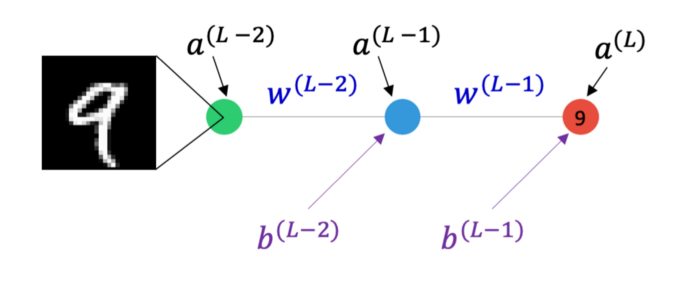
\includegraphics[width=\linewidth]{pictures/backpropagation/1-1-1_network.png}
		\caption{простейшая нейронная сеть}
		\label{simplest_nn}
	\end{figure}
	
	На рисунке \ref{simplest_nn} изображена простейшая нейронная сеть, где зелёный, синий и красный нейрон отвечают за входной, скрытый и выходной нейрон (слой, если говорить в терминах более крупных нейронных сетей) соответственно. Обозначим функцию активации последнего нейрона как $a^{(L)}$, функцию активации предпоследнего слоя как $a^{(L-1)}$, а функцию активации первого слоя как $a^{(L-2)}$, где $L$ - количество слоёв в нашей нейронной сети (в нашем случае $L=3$). Аналогично определим веса и биасы между слоем $L-1$ и $L$ как $w^{(L-1)}$ и $b^{(L-1)}$.
	
	Представим, что наша картинка цифры $9$ состоит из одного пикселя (понятно, что это не возможно; сделаем это для упрощения вычислений). Теперь, пусть после того, как этот один пиксель прошёл через все три слоя нашей простейшей нейронной сети (стадия прямого распространения), на выходе мы получили число 0.68 (так как мы решаем задачу классификации, то выходные значения должны находиться в диапазоне от 0 до 1, что можно интерпретировать как вероятность; для этого можно в качестве функции активации последнего слоя (в нашем случае нейрона) использовать функцию Softmax (добавить сюда потом ссылку)). Но наше желаемое выходное значение --- это 1 (т.е. мы хотим (после завершения обучения), чтобы наша сеть была уверена на 100\%, что данная картинка (в нашем случае один пиксель) --- это число 9). Теперь, пусть мы будем использовать средне квадратичную ошибку в качестве функции потерь. Т.е. мы получаем, что потеря $C$ для одного тренировочного образца (т.е цифры 9) равняется $(0.68-1)^2$
	
	\subsection{Слой $L-1$}
	
	Рассчитаем градиент нашей функуии потерь $C$ учитывая вес, соединяющий нейроны в слое $L$ со слоем $L-1$. Чтобы посмотреть, как бы мы это сделали, развернём последний слой нашей простейшей нейронной сети.
	
	\begin{figure}[h!]
		\centering
		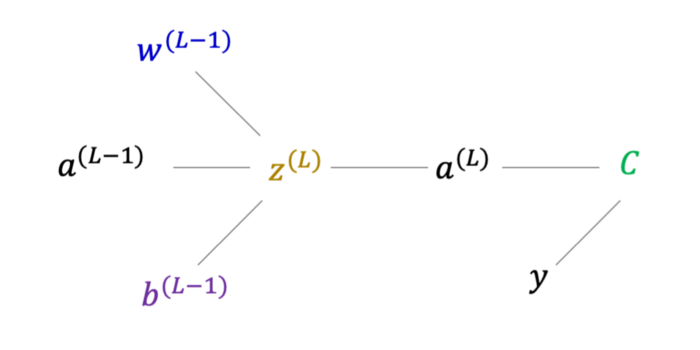
\includegraphics[width=\linewidth]{pictures/backpropagation/last_layer.png}
		\caption{Последний слой}
		\label{last_layer}
	\end{figure}
	
	Фигура \ref{last_layer} показывает, как каждый параметер последних двух слоёв влияет на потерю $C$. Чтобы получить взвешенную сумму $z^{(L)}$ для последнего слоя, мы умножаем активацию слоя (т.е. выход предпоследнего слоя, к которому была применена соответствующая функция активации для даного слоя) $L-1$ на вес $w^{(L-1)}$, соединяющий два слоя, а затем мы прибавляем биас $b^{(L-1)}$. И наконец, мы пропускаем взвешенную сумму через нелинейную функцию (функцию активации) $\sigma(z^{(L)})$, чтобы посчитать $a^{(L)}$.
	
	\begin{figure}[h!]
		\centering
		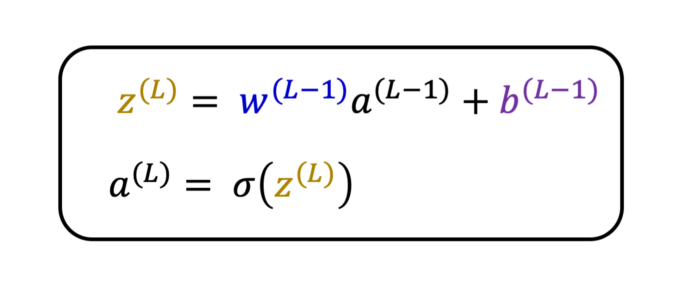
\includegraphics[width=\linewidth]{pictures/backpropagation/sigma.png}
		\caption{Функция активации}
		\label{weighted_sum}
	\end{figure}

	Теперь мы хотим посмотреть, как сильно изменится $C$, если мы изменим $w^{(L-1)}$. Т.е. мы хотим посчитать $\dfrac{\partial C}{\partial w^{(L-1)}}$.
	
	\begin{figure}[h!]
		\centering
		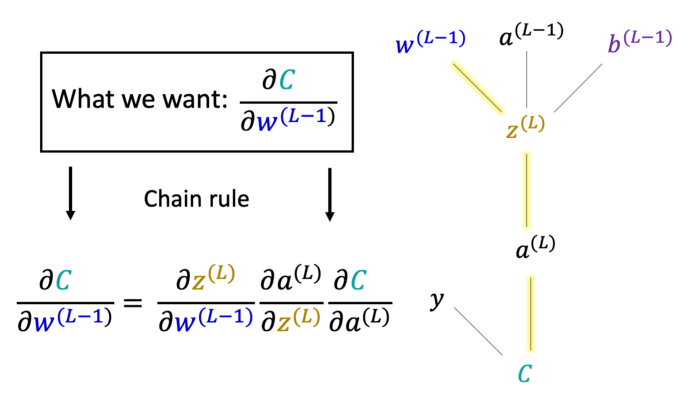
\includegraphics[width=\linewidth]{pictures/backpropagation/chain_rule.png}
		\caption{Дифференцирование}
		\label{derivative_1}
	\end{figure}

	Из картинки \ref{derivative_1} можно понять, как вес $w^{(L-1)}$ влияет на $C$. Сначала вес $w^{(L-1)}$ даёт вклад во взвешенную сумму $z^{(L)}$, которая используется для того, чтобы посчитать потерю $C$. Найдём частную производную $\dfrac{\partial C}{\partial w^{(L-1)}}$ явно.
	
	\begin{figure}[h!]
		\centering
		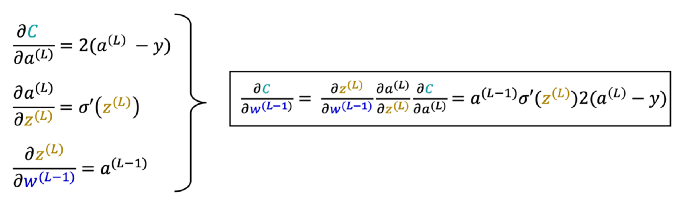
\includegraphics[width=\linewidth]{pictures/backpropagation/derivative_itself.png}
		\caption{Находим частную производную явно}
		\label{derivative_itself_weight}
	\end{figure}

	То, как получены последние два выражения в левой части - очевидно. Рассмотрим первое. Так как для подсчёта потери мы используем средне квадратичную ошибку (MSE, которая считается как $(a^{(L)}-y)^2$), то если взять от этого производную по $\partial a^{(L)}$, то мы как раз получим $2(a^{(L)}-y)$.
	
	Заметим, что мы не нашли производную от нашей функции активации (которую мы обозначили как $\sigma$) явно. Если бы мы использовали Sigmoid в качестве нашей функции активации:
	
	\[\dfrac{1}{1+e^{-z}}\]
	
	Тогда её производная равнялась бы:
	
	\[\dfrac{e^{-z}}{(1+e^{-z})^2}\]
	
	\textbf{Замечание:} вот почему важно использовать в качестве функций активации всюду дифференцируемые функции, в противном случае мы не сможем рассчитать наши градиенты, однако функцию ReLu всё же можно использовать (добавить потом сюда ссылку).
	
	Также мы хотим знать, как изменится значение нашей функции потерь, если мы изменим биас $b^{(L-1)}$.
	
	\begin{figure}[h!]
		\centering
		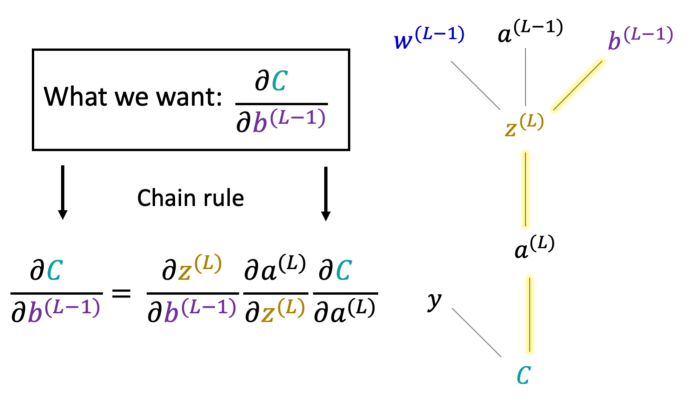
\includegraphics[width=\linewidth]{pictures/backpropagation/bias.png}
		\caption{Считаем производную для биаса}
		\label{derivative_bias}
	\end{figure}
	
	Как можно заметить, поменялся только первый множитель. Аналогично, найдём явную производную.
	
	\begin{figure}[h!]
		\centering
		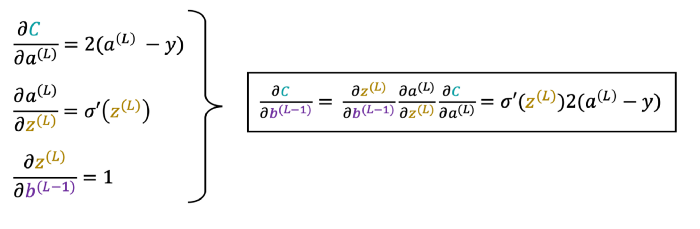
\includegraphics[width=\linewidth]{pictures/backpropagation/derivative_itself_bias.png}
		\caption{Считаем производную для биаса}
		\label{derivative_itself_bias}
	\end{figure}

	Отлично, теперь нейронная сеть может использовать полученные выражения для обновления весов и биасов по следующему принципу.

	\begin{figure}[h!]
		\centering
		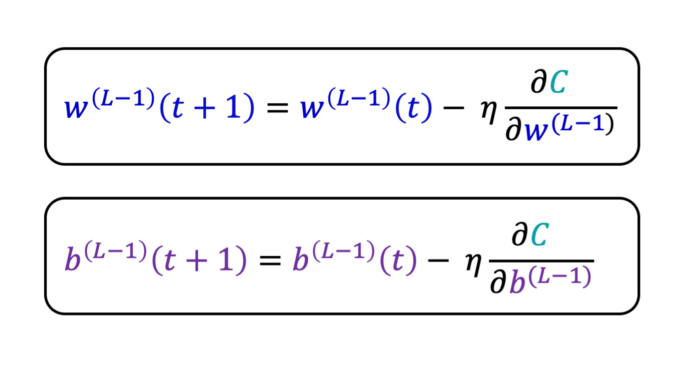
\includegraphics[width=\linewidth]{pictures/backpropagation/updating.png}
		\caption{Обновление весов}
		\label{updating}
	\end{figure}

	На картинке \ref{updating} $\eta$ --- это learning rate.
	
	Несмотря на то, что нейронная сеть не имеет прямого контроля над $a^{(L-1)}$, скоро будет показано, что что нам будет это нужно, чтобы дальше двигаться по сети и обновлять параметры, поэтому проделаем предыдущие шаги, только для $a^{(L-1)}$.
	
	Получаем:
	
	\begin{figure}[h!]
		\centering
		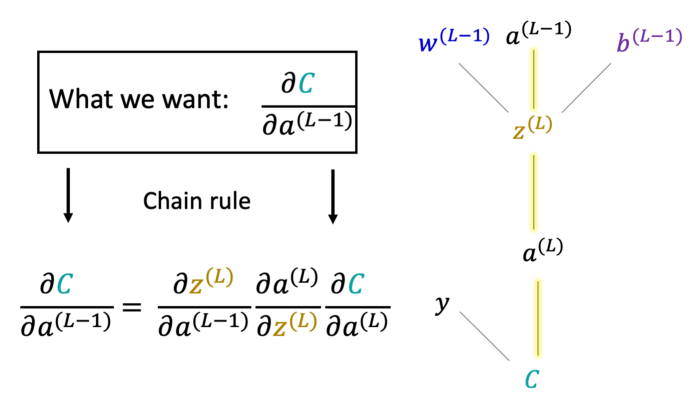
\includegraphics[width=\linewidth]{pictures/backpropagation/last_activation.png}
		\caption{Считаем градиент относительно функции активации предпоследнего слоя}
		\label{last_activation}
	\end{figure}

	Находим производную явно:
	
	\begin{figure}[h!]
		\centering
		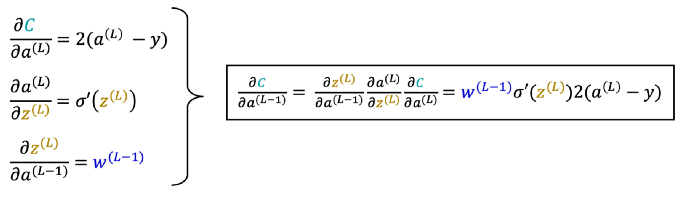
\includegraphics[width=\linewidth]{pictures/backpropagation/last_activation_itself.png}
		\caption{Находим производную явно}
		\label{last_activation_itself}
	\end{figure}

	\subsection{Слой $L-2$}
	
	Теперь давайте посмотрим, как будет меняться значение функции потерь $C$, если изменять параметры в слое $L-2$. Как и раньше, нарисуем граф, чтобы наглядо продемонстрировать, как $w^{(L-2)}$ и $b^{(L-2)}$ косвенно влияют на значение потери $C$.
	
	\begin{figure}[h!]
		\centering
		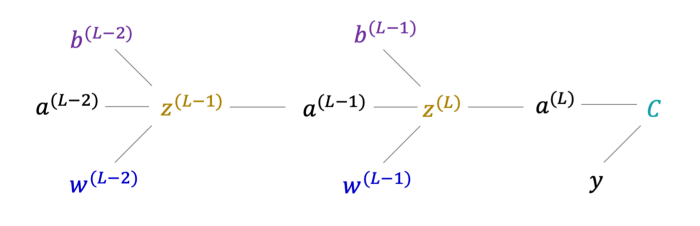
\includegraphics[width=\linewidth]{pictures/backpropagation/first_layer.png}
		\caption{Слои $L-1$ и $L-2$}
		\label{first_layer}
	\end{figure}

	Аналогично, используя цепное правило, посмотрим, как изменение веса $w^{(L-2)}$ влияет на значение функции потерь $C$.
	
	\begin{figure}[h!]
		\centering
		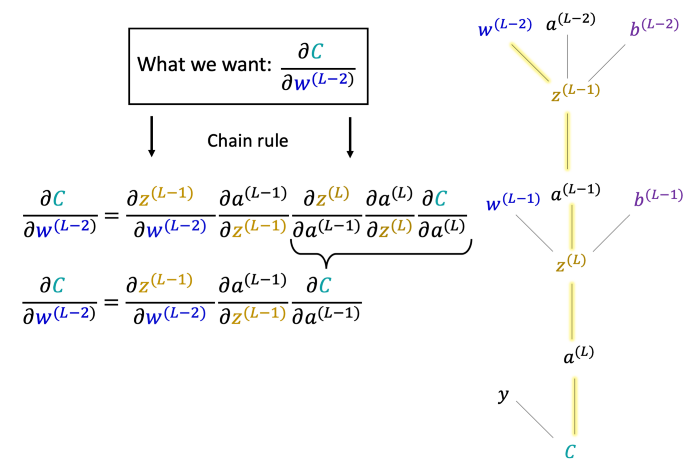
\includegraphics[width=\linewidth]{pictures/backpropagation/first_layer_weight.png}
		\caption{Частная производная для веса первого слоя}
		\label{first_layer_weight}
	\end{figure}

	Теперь найдём производную явно:
	
	\begin{figure}[h!]
		\centering
		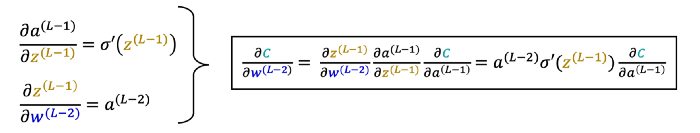
\includegraphics[width=\linewidth]{pictures/backpropagation/first_layer_itself.png}
		\caption{Производная в явном виде}
		\label{first_layer_itself}
	\end{figure}
	
	Аналогичным образом можно посчитать градиенты для всех весов и биасов. Этот алгоритм называется \textbf{обратным распространением ошибки}.
	
	
	
	











	
	
	
	
	
	
	 
\end{document}